\documentclass[12pt]{exam}

\usepackage[margin=0.5in]{geometry}
\usepackage{amsmath,amssymb}
\usepackage{tikz,soul}
\usepackage{diagbox}
\usetikzlibrary{arrows,automata,positioning}

\newcommand{\ds}{\displaystyle}
\newcommand{\bs}{\backslash}
\newcommand{\on}{\operatorname}
\newcommand{\R}{\mathbb{R}}
\newcommand{\Z}{\mathbb{Z}}
\newcommand{\N}{\mathbb{N}}

\begin{document}
\pagestyle{empty}
\subsubsection*{Homework 7 - Computer Science 461 \hfill Name: \underline{\hspace*{2in}}}

\textit{Due Monday, March 17.} % You can e-mail your code for the computer programming problems to me at }\verb|blins@hsc.edu|.

\begin{questions}

\question Identify the context-free language that is accepted by each of the following pushdown automata (PDA).  Explain (briefly) you answer for each.
\begin{parts}
\part 
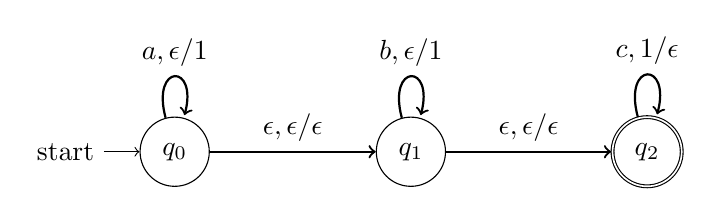
\begin{tikzpicture}[node distance=3cm,auto]
  \node[state,initial]   (q_0)                 {$q_0$};
  \node[state]           (q_1) [right of=q_0]  {$q_1$};
  \node[state,accepting] (q_2) [right of=q_1]  {$q_2$};
  \path[thick,->]
  (q_0) edge [loop above] node {$a, \epsilon/1$} ()
  (q_0) edge              node {$\epsilon, \epsilon/\epsilon$} (q_1)
  (q_1) edge              node {$\epsilon, \epsilon/\epsilon$} (q_2)
  (q_1) edge [loop above] node {$b, \epsilon/1$} ()
  (q_2) edge [loop above] node {$c, 1/\epsilon$} ();
\end{tikzpicture}

\begin{solution}
$$L = \{a^m b^n c^{m+n} : m, n \in \N \}$$
\end{solution}
\vfill

\part 
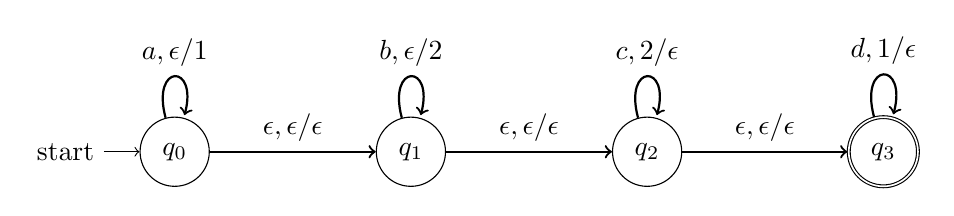
\begin{tikzpicture}[node distance=3cm,auto]
  \node[state,initial]   (q_0)                 {$q_0$};
  \node[state]           (q_1) [right of=q_0]  {$q_1$};
  \node[state]           (q_2) [right of=q_1]  {$q_2$};
  \node[state,accepting] (q_3) [right of=q_2]  {$q_3$};
  \path[thick,->]
  (q_0) edge [loop above] node {$a, \epsilon/1$} ()
  (q_0) edge              node {$\epsilon, \epsilon/\epsilon$} (q_1)
  (q_1) edge [loop above] node {$b, \epsilon/2$} ()
  (q_1) edge              node {$\epsilon, \epsilon/\epsilon$} (q_2)
  (q_2) edge [loop above] node {$c, 2/\epsilon$} ()
  (q_2) edge              node {$\epsilon, \epsilon/\epsilon$} (q_3)
  (q_3) edge [loop above] node {$d, 1/\epsilon$} ();
\end{tikzpicture}

\begin{solution}
$$L = \{a^m b^n c^n d^m : m, n \in \N \}$$
\end{solution}
\vfill



\part 
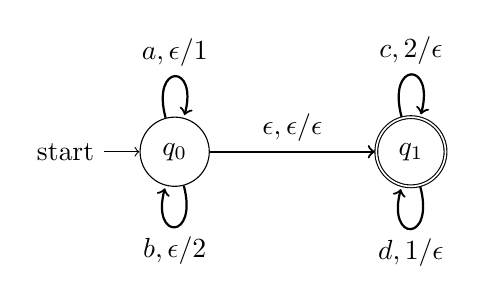
\begin{tikzpicture}[node distance=3cm,auto]
  \node[state,initial]   (q_0)                 {$q_0$};
  \node[state,accepting] (q_1) [right of=q_0]  {$q_1$};
  \path[thick,->]
  (q_0) edge [loop above] node {$a, \epsilon/1$} ()
  (q_0) edge [loop below] node {$b, \epsilon/2$} ()
  (q_0) edge              node {$\epsilon, \epsilon/\epsilon$} (q_1)
  (q_1) edge [loop above] node {$c, 2/\epsilon$} ()
  (q_1) edge [loop below] node {$d, 1/\epsilon$} ();
\end{tikzpicture}

\begin{solution}
Strings in $\{a,b\}^*$ concatenated with strings in $\{c,d\}^*$ that have the same number of $a's$ and $d's$ and the same number of $b$'s and $c$'s. 
\end{solution}
\vfill
\end{parts}

\question Let $\Sigma = \{ \verb|(,),[,]| \}$. That is, $\Sigma$ is the alphabet consisting of the four symbols \verb|(|, \verb|)|, \verb|[|, and \verb|]|. Let $L$ be the language over $\Sigma$ consisting of strings in which both parentheses and brackets are balanced. For example, the string \verb|([][()()])([])| is in $L$ but \verb|[(])| is not. Find a PDA that accepts this language. Hint: \emph{you should only need one state!}
\vfill
\vfill
\vfill




\newpage


\question Use the pumping lemma to prove that the language $\{a^n b^n a^n b^n : n \in \N \}$ is not context-free. 
\begin{solution}
Let $s = a^p b^p a^p b^p$.  Then the substring in $vxy$ in $s$ can is either contained in a substring with either a single letter or a substring that begins with one letter and ends with a different one.  In either case, when you pump $v$ and $y$, you will increase the number of $a$'s and $b$'s in at most two of the blocks of $p$ letters that are the same.  That will immediately make a string that is not in the language so the language is not context-free. 
\end{solution}
\vfill

%\part $\{w_1 w_2 : w_1 w_2 \in \{a,b\}^* \text{ and } w_1 \text{ is a substring of } w_2 \}$.
%\begin{solution}
%NOT SURE THIS ONE WORKS WITHOUT A DIVIDER CHARACTER B/W w_1 and w_2
%\end{solution}
\question Is the language $\{a^m + a^n = a^{m+n} : m, n \in \N \}$ over the alphabet $\Sigma = \{a, +, = \}$ context-free?  Explain why or why not.
\begin{solution}
Yes, it is context free.  You can generate this language with the grammar 
\begin{align*}
S &\rightarrow aSa \\
S &\rightarrow +T \\
T &\rightarrow aTa \\
T &\rightarrow =
\end{align*}
\end{solution}
\vfill


\question For any languages $A$ and $B$, let $A \diamond B = \{ xy : x \in A, y\in B, \text{ and } |x| = |y| \}$. If $A$ and $B$ are regular languages, prove that $A \diamond B$ is a context-free language by describing how you could use NFAs for $A$ and $B$ to construct a PDA for $A \diamond B$.   
\begin{solution}
Since both $A$ and $B$ are regular, there are NFAs $M_A$ and $M_B$ that recognize $A$ and $B$ respectively. Create an PDA $N_A$ that is identical to $M_A$, but it pushes an $a$ on the stack each time it reads a symbol in $\Sigma$. Then create an PDA identical to $M_B$ except it pops an $a$ off the stack each time it reads a symbol.  You can run the PDA corresponding to $M_A$, and each time it reaches an accept state, you can apply an $\epsilon$ transition to activate the start state in the PDA corresponding to $M_B$.  If this combined PDA reaches the end of the input string with an empty stack, then you will know that we have a string that is a concatenation $xy$ with $|x| = |y|$ and $x \in A$, $y \in B$. 
\end{solution}
\vfill

%%%% THIS NEXT ONE IS MAYBE TOO EASY FOR THE HOMEWORK?!?! IS IT CRAZY TO THINK THAT. INSTEAD IT MIGHT MAKE A GOOD TEST QUESTION.
%\question For any language $A \subseteq \Sigma^*$, define a new language
%$$\on{ENDS-IN}(A) = \{ v w : v \in \Sigma^*, w \in A \}.$$
%If $A$ is context-free, then prove that $\on{ENDS-IN}(A)$ is also context free. 
%
%\vfill

\end{questions}
\end{document}
